{\color{red}Some lead into here.}

\section{Summary of Methods}

\begin{table}
\caption{Summary of Partitioning Methods}
\label{8_methods}
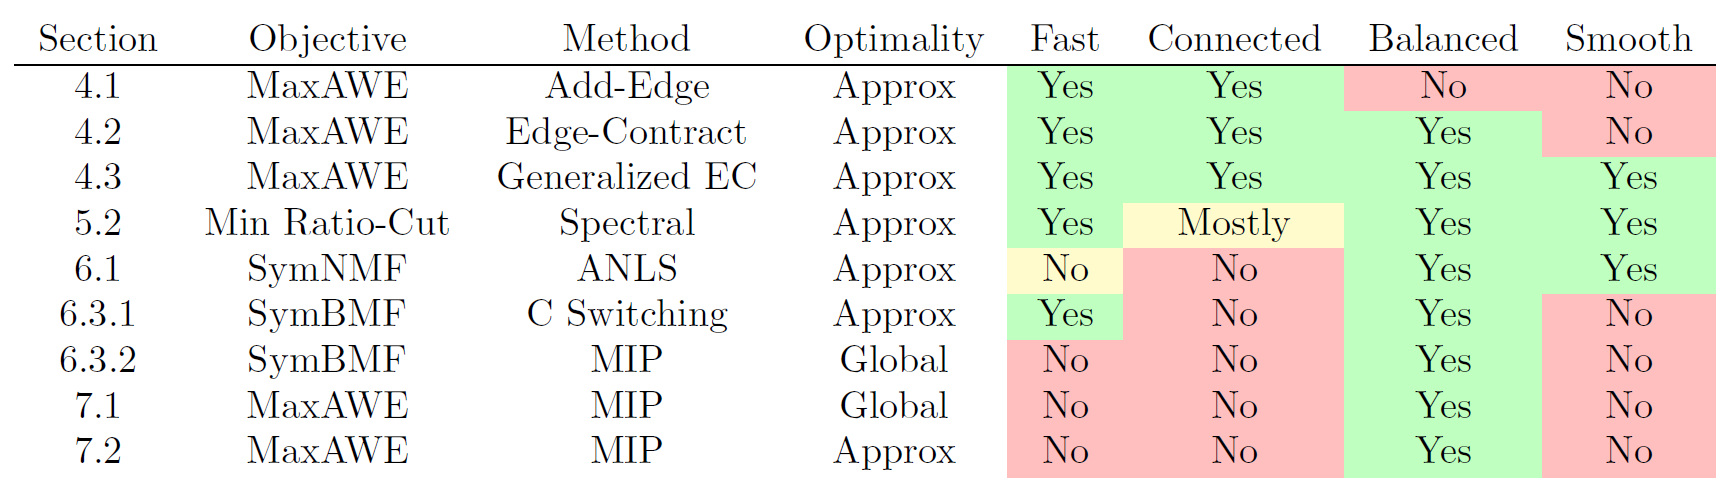
\includegraphics[scale = 0.5]{figs/8_methods.png}
%\begin{tabular}{cccccccc}
%Section & Objective & Method & Optimality & Fast & Connected & Balanced & Smooth \\
\hline
4.1 & MaxAWE & Add-Edge & Approx & \cellcolor{green!25}Yes & \cellcolor{green!25}Yes & \cellcolor{red!25}No & \cellcolor{red!25}No \\
4.2 & MaxAWE & Edge-Contract & Approx & \cellcolor{green!25}Yes & \cellcolor{green!25}Yes & \cellcolor{green!25}Yes & \cellcolor{red!25}No \\
4.3 & MaxAWE & Generalized EC & Approx & \cellcolor{green!25}Yes & \cellcolor{green!25}Yes & \cellcolor{green!25}Yes & \cellcolor{green!25}Yes \\
5.2 & Min Ratio-Cut & Spectral & Approx & \cellcolor{green!25}Yes & \cellcolor{yellow!25}Mostly & \cellcolor{green!25}Yes & \cellcolor{green!25}Yes \\
6.1 & SymNMF & ANLS & Approx & \cellcolor{yellow!25}No & \cellcolor{red!25}No & \cellcolor{green!25}Yes & \cellcolor{green!25}Yes \\
6.3.1 & SymBMF & C Switching & Approx & \cellcolor{green!25}Yes & \cellcolor{red!25}No & \cellcolor{green!25}Yes & \cellcolor{red!25}No \\
6.3.2 & SymBMF & MIP & Global & \cellcolor{red!25}No & \cellcolor{red!25}No & \cellcolor{green!25}Yes & \cellcolor{red!25}No \\
7.1 & MaxAWE & MIP & Global & \cellcolor{red!25}No & \cellcolor{red!25}No & \cellcolor{green!25}Yes & \cellcolor{red!25}No \\
7.2 & MaxAWE & MIP & Approx & \cellcolor{red!25}No & \cellcolor{red!25}No & \cellcolor{green!25}Yes & \cellcolor{red!25}No \\

%\end{tabular}
\end{table}

Table (\ref{8_methods}) summarizes the objectives, advantages, and
drawbacks of each partitioning method we've presented in the previous
chapters. Clearly, the requirement of parcels to be connected components
is the biggest roadblock to developing a good method.

There is a post-processing method that can take a parcellation with
disconnected components and modify it to be connected. The method is to
treat each separate component of a parcel as new parcels, create a
Contractible Graph with these new parcels as components, and apply the
(Generalized) Edge Contract algorithm. This was carried out as a
post-processing step in the spectral and SymBMF parcellations, detailed
in the next section.

The second limiting factor is computational time. The Alternating
Nonnegative Least Squares algorithm can be made to work on graphs as
large as the brain, but this would require some specialized data
structures for the computation of $X$ and $Y$ to avoid re-computing
unchanged columns. Unfortunately we did not have enough time to
implement this.

The problem of computational time is most evident in the integer (and
linear) programming methods. The fact that our brain data was too large
for even the lightest linear program shows that this generic
optimization approach is typically not feasible. However, these
proposed methods may be of use to problems with smaller data sets.

One possible approach to dealing with computational time that we have
not had the time to explore is to apply the MIP methods to small
subgraphs of the brain. For instance, one could take the AAL
parcellation and obtain a finer parcellation by using a MIP method on
each of the AAL parcels.

The only method that satisfies the requirements of computational speed,
parcel connectedness, size balance, and smoothness without any
post-processing steps is the Generalized Edge-Contraction family of
algorithms. In the next section we will show that it is also the
parcellation method that produces the best Adjacent-Scores.

All of the methods above can be applied to the similar problem of
\textit{clustering}. In fact, similarity-based clustering is just a
special case of graph partitioning where the graph is fully connected
(i.e., every vertex has an edge to every other vertex), so connectedness
of partitions is no longer a relevant factor. Then, if we define the
Adjacent-Score in terms of similarity equal to negative Euclidean
distance squared
\[ \frac{1}{K}\sum_{k=1}^K \frac{1}{{|V_k| \choose 2}}
   \sum_{x,y \in V_k} - \|x - y\|^2, \]
the objective of maximizing Adjacent-Score becomes equivalent to 
minimizing a weighted within-cluster sum of squares objective
\[ \sum_{k=1}^K \frac{1}{{|V_k| \choose 2}}
   \sum_{x \in V_k} \|x - \mu_k\|^2 \]
where $\mu_k$ is the mean of all $x$ in $V_k$.

{\color{red}It'll be nice to cite the equations in Chapter 3 for
the criterion values}

\section{Parcellations of ABIDE fMRI Scans}

\begin{table}
\caption{Criteria Scores of Various Parcellation Methods, %
Averaged Across Normal Brains}
\label{normal}
\begin{tabular}{l | r r r r r r}
& \rot{Adjacent}
& \rot{Boundary}
& \rot{RatioCut}
& \rot{CompParc}
& \rot{Balance}
& \rot{Jaggedness}
\\ \hline
GenEC (3,1)         & 0.766 & 0.799 & 47.118 & 1     & 0.251 & 23.930 \\
GenEC (6,1)         & 0.774 & 0.796 & 51.342 & 1     & 0.280 & 28.801 \\
GenEC (6,4)         & 0.773 & 0.800 & 51.285 & 1     & 0.335 & 29.199 \\
Spectral            & 0.747 & 0.810 & 43.242 & 1.027 & 0.728 & 16.347 \\
Spectral GenEC(6,4) & 0.747 & 0.810 & 43.162 & 1     & 0.713 & 16.305 \\
SymBMF      & 0.845 & 0.962 & 293.662 & 470.994 & 0.838 & 305.302 \\
SymBMF GenEC(6,4)   & 0.773 & 0.798 & 53.256 & 1     & 0.290 & 30.086 \\

\end{tabular}
\end{table}

\begin{table}
\caption{Criteria Scores of Various Parcellation Methods, %
Averaged Across Autism Spectrum Brains}
\label{autism}
\begin{tabular}{l | r r r r r r}
& \rot{Adjacent} & \rot{Boundary} & \rot{RatioCut} & \rot{CompParc} & \rot{Balance} & \rot{Jaggedness} \\
\hline
GenEC (3,1) & 0.762 & 0.821 & 46.615 & 1 & 0.210 & 25.008 \\
GenEC (6,1) & 0.769 & 0.827 & 51.613 & 1 & 0.249 & 31.178 \\
GenEC (6,4) & 0.771 & 0.821 & 51.705 & 1 & 0.309 & 31.821 \\
Spectral    & 0.739 & 0.827 & 42.464 & 1.024 & 0.697 & 16.36 \\
Spectral GenEC(6,4) & 0.739 & 0.827 & 42.427 & 1 & 0.677 & 16.333 \\
SymBMF & 0.844 & 0.969 & 289.129 & 473.102 & 0.827 & 306.992 \\
SymBMF GenEC(6,4) & 0.769 & 0.821 & 52.742 & 1 & 0.261 & 31.927 \\

\end{tabular}
\end{table}

Tables (\ref{normal}) and (\ref{autism}) respectively show the results
of various parcellation methods carried out on resting state fMRI scans
of 6 control and 6 autism patients. The number of parcels in each
method is set to 116, the same as AAL. Each brain was preprocessed to
remove vertices with edge weights of 0 to all adjacent vertices. For
each method and criterion, the values are averaged over the six 
subjects in each cohort. In our methods, SymBMF was carried out using
component switching on the incomplete adjacency matrix (only
approximation of non-zero entries in the $A$ matrix was considered).
GenEC ($\alpha$, $\beta$) denotes a Generalized Edge-Contract
algorithm using standard priority function (\ref{priority_func}) with
parameters $\alpha$ and $\beta$. When this is written after a different
method such as Spectral, it means we post-processed the Spectral
parcellation using GenEC to obtain connected parcels.

Despite producing a parcellation with the highest Adjacent-Score, the
Component Switching SymBMF method is the least suitable for parcellation
since its parcels are extremely fragmented, with an average 473
components per parcel. The reason for this is that the adjacency matrix
was treated as incomplete, so there was no penalty for a vertex
belonging to a parcel with many vertices it is disconnected from.
The high Adjacent-Score of SymBMF parcellations suggests a trade-off
between maximizing weights of within edges and creating connected and
smooth parcels.

The other parcellations aside from pure SymBMF has CompParc, Balance,
and Jaggedness scores that were at least as good as the AAL ones.
The Spectral parcellations were the smoothest, as expected, but this
came at the cost of lower Adjacent-Score and higher Boundary-Score
relative to the GenEC parcellations.
In both groups, the Generalized Edge-Contract with parameters
$\alpha = 6$ and $\beta = 4$ performed best. These parcellations had
the highest Adjacent-Scores and while maintaining Balance and
Jaggedness Scores close to those of the AAL. There is no significant
difference in the parcellation results of autism and control brains.

\section{Reproducibility of Parcellations and Cross-Validation}

\begin{figure}
\caption{Adjusted Rand Index Between Different 116-Parcel %
Parcellations of the same fMRI Scan, Averaged over All Subjects}
\label{ari_same}
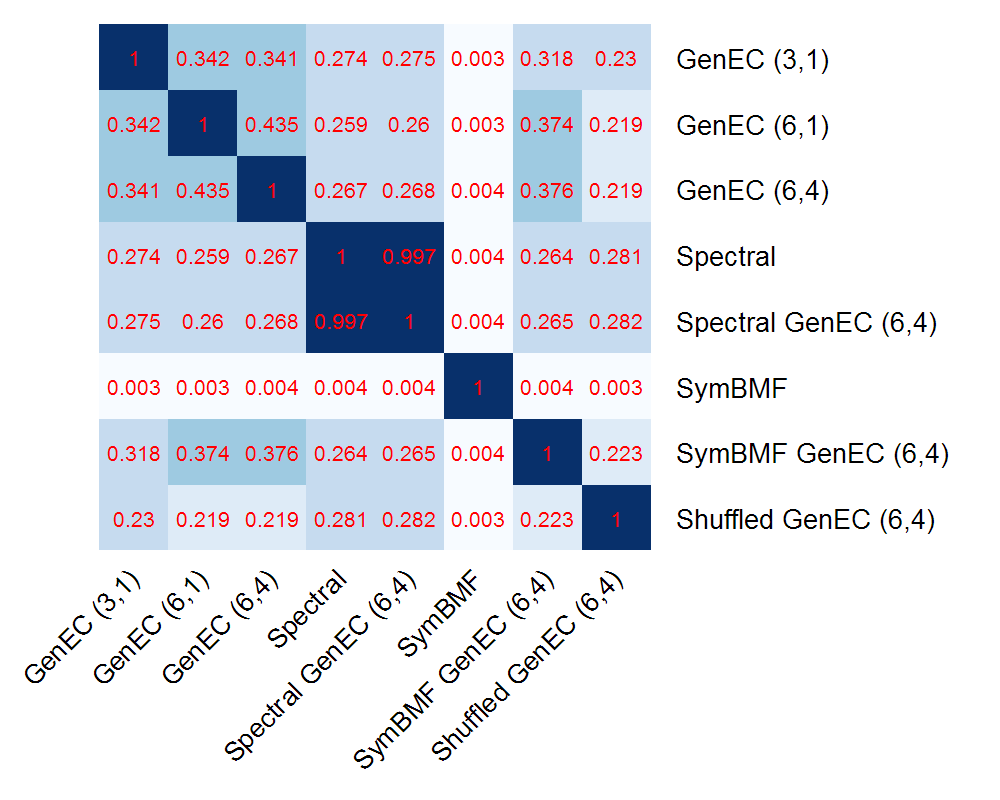
\includegraphics[scale = 1]{figs/8_ari_same.png}
\end{figure}

\begin{figure}
\caption{Adjusted Rand Index Between 116-Parcel GenEC(6,4)
Parcellations on Different fMRI Scans}
\label{ari_diff}
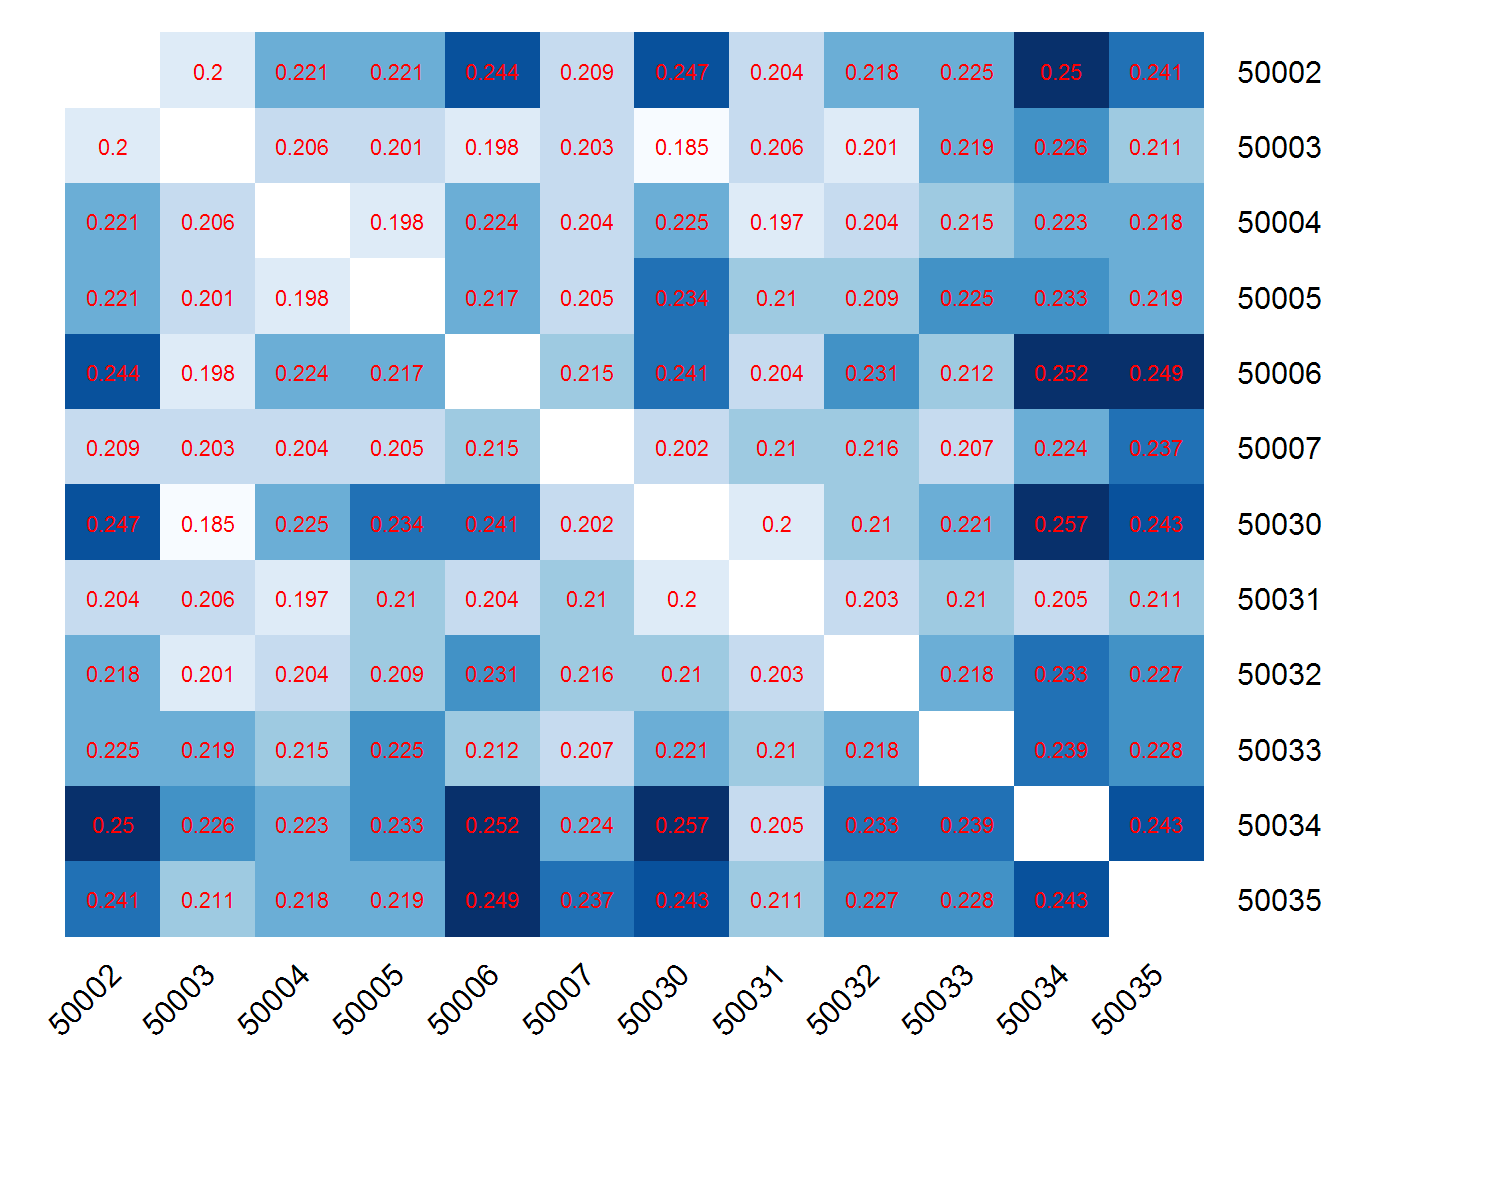
\includegraphics[scale = 0.95]{figs/8_ari_diff.png}
\end{figure}

We measured the similarity of 116-parcel parcellations from different
methods on the same brain, across brains in the control and autistic
cohorts. We used the Adjusted Rand Index \ref{ari} {\color{red}Citation doesn't
work} as our measure of
similarity, where 1 means identical parcel assignments and 0 means no
different from random parcel assignments. The result is shown in Figure
(\ref{ari_same}). The last row and column refer to ARI values with
respect to a random parcellation, generated by applying GenEC (6,4) to
the same brain graph with edge weights shuffled. The reason for this is
to account for the portion of ARI scores that derive solely from the
connectedness and smoothness property of parcellations.

As expected, the first three GenEC parcellations are similar to one
another, more than they are to the shuffled parcellation or to the
Spectral parcellations. The SymBMF GenEC (6,4) parcellation can also be
grouped with the first three. The unconnected SymBMF parcellation is
similar to no other since it is too fragmented.

Next, we restricted ourselves to the GenEC (6,4) method and measured
how similar the parcellations this method produced on different brains
are. The results are shown in Figure (\ref{ari_diff}). From Figure
(\ref{ari_same}) we know that the ARI between a GenEC (6,4) parcellation
on a shuffled brain graph and an actual one is around 0.219.
Surprisingly, for nearly all pairs of brains, the ARI value between
their GenEC (6,4) parcellations is no greater than this. We also see
that the mean ARI between autistic and control brains is not
significantly different from the mean ARI between brains of the same
cohort at the 116-parcel level. This suggests too much variation in the
spatial distribution of distance correlations across the edges of
different brain graphs for there to be a common parcellation fitting
all brains.

\begin{figure}
\caption{Adjacent-Score Minus Mean Edge Weight Cross-Validation of
116-Parcel GenEC (6,4) Parcellation on 12 Autism and Control Brains}
\label{cv_ec}
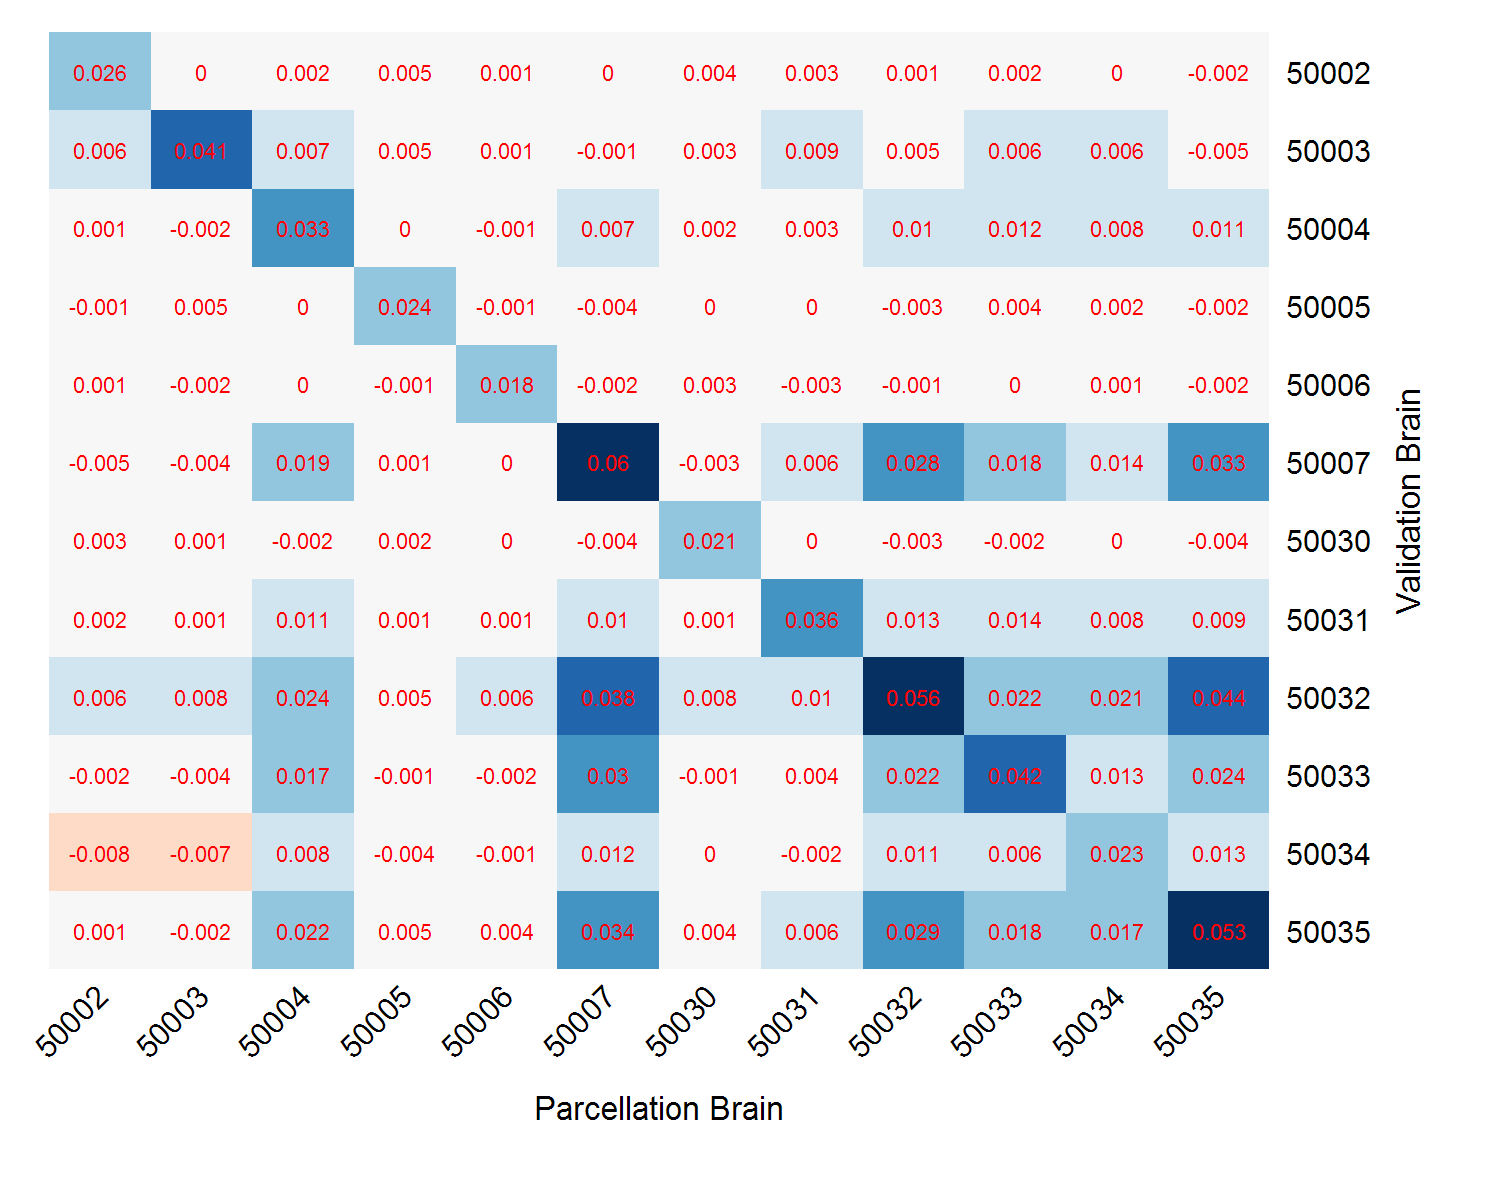
\includegraphics[scale = 1]{figs/8_cv_ec.png}
\end{figure}

To test this hypothesis, we conducted a cross-validation procedure where
for each pair of brains, we parcellated one using GenEC (6,4) and
computed the Adjacent-Score of the resulting parcellation on the
\textit{other} brain. From this Adjacent-Score we subtracted the mean
edge weight on the test brain and display the resulting 12 by 12 matrix
in Figure (\ref{cv_ec}).

Brains labeled 50030 and greater are control brains. It is interesting
that cross-validation scores within the control cohort are higher than
those between the two cohorts and those within the autistic cohort.
Further investigation is needed to determine if this result is
significant.

Finally, we investigate whether both the low Adjusted Rand Index and
cross-validation scores between parcellations of different brains could
be due to overfitting. The GenEC methods produced parcellations that
scored well in-sample but very poorly out-of-sample, so it is possible
that the parcellations they produce are too flexible. To see if this
could be the case, we perform the same cross-validation procedure
except now using the spectral method (with GenEC (6,4) post-processing
to ensure parcel connectedness). Partitions obtained via the spectral
method are smoother, and thus are less likely to overfit the
Adjacent-Score.

\section{Conclusion}


{\color{red}Some things to think about: Future Work, general thoughts about
parcellation, which methods did you expect to do well and which actually did
well.}
